\paragraph{}
For this part, let's talk about a whole different beast : The software. This correspond to all of the code executed
on the microcontroller to command all of the actions done, from the control of the rocket trajectory to the log of
the temperature !

\paragraph{}
This is a very complex topic, that could be the subject of a whole report, so we're forced to reduce some part of it.
Nonetheless, we'll go trough all of the main subjects.
First, we'll talk about the configuration of the different functions by exploring the different devicetree files.
In a second time, we'll go trough the fundamentals of Zephyr RTOS, which was used to schedule main tasks and handle
the nasty memory stuff for ourselves.
Then, we'll start to ramp up into the different abstraction layers used, from the drivers to the threads.
To conlude this chapter, we're going to show the global software architecture we used over the project.

% Including all of the files
% Device trees
\section{Introduction to devicetrees}
First, we need to explain what is a devicetree, because that's actually far from begin clear and easy to understand.
The wikipedia article describe it concisely, here a quotation :

    \quote{In computing, a devicetree (also written device tree) 
    is a data structure describing the hardware components of 
    a particular computer so that the operating system's kernel 
    can use and manage those components, including the CPU or CPUs, 
    the memory, the buses and the integrated peripherals.}
    \cite{devicetree}

\paragraph{}
So, we know that we're going to found some hardware description in theses files. Theses kind of files are 
commonly used on the Linux kernel for this purpose, on hardware that is much faster than our small 
microcontroller. 
This way of describing hardware, even if it's quite difficult to get it rigth enable some extremely smart
options, such as dynamic reconfiguration.

\paragraph{}
In fact, for other controllers we're supposed to bind pins by hand by correctly assigning register values.
This is easy to develop, but once you want to change something, it become difficult to not make mistake by 
misreading a value.
This problem is solved with devicetrees, since they store hardware config for ourselves. And, they can 
even store multiple configuration, and offer the option to switch at compile time.

It's then possible to develop a devicetree for the development board, and for the final board, and within
one parameter change between them !

\paragraph{}
Devicetrees are written in plain text, and there can be only a single file used for the compilation at 
a given time. Theses files use the extension ".dts". This main file contain the root, also named "/", 
as any UNIX filesystem. Then, we add "folders", which are named nodes to it. Nodes can be 
nested inside others to make the code cleaner. Theses are sometimes called sub-nodes. And inside nodes, 
there is some properties, that can be seen as a variable that configure one aspect.

As an example, a node may be RAM, and properties are the size, the speed and any other hardware
parameters.

In correctly designed devicetrees, there shall be one node for each device that can't be detected on 
runtime. This include I2C slaves.

\paragraph{}
We can easily image that theses files will become big, even for simple systems. To give an idea, there is
arround one thousand of lines just for our simple microcontroller !

Thus, the developpers of Device Tree Compilers managed to create an include syntax, based on overlays files
(".dts\textbf{i}"). Theses are included by after and contain only the code for a single peripheral.
Then, we include them over the main devicetree file. 

If the new nodes were not present, they're added to the main code. If they were already existing, the new 
file will overhide properties. 
It's always the latest added that take the priority.




\section{Configuration using devicetrees}
Since we're using a microcontroller that is widely available, most of the work with 
devicetrees has already been done by the manufacturer.

Thus, we don't need to care about memory, cpus, or other internals details of the
peripherals. We only enable and configure the required peripherals.

\paragraph{}
To make the structure cleaner, we've used a lot of overlays, because it's much easier
to debug and find the right property when needed.

\subsection{Main overlays}

\subsection{Peripherals overlays}
\subsubsection{PWM configuration}
\subsubsection{I2C configuration}

% Zephyr
\input{chapters/prog/zephyr/rtos.tex}
\section{Zephyr RTOS}
As we seen just before, RTOS may be very usefull to create complex programs on CPUs.
Since we're using Zephyr, let's dig a bit deeper into this RTOS.

\subsection{Configuration}
As we seen previously, Zephyr isn't based on pure code to configure the device. It used 
a lot of others files, including devicetrees to describe the hardware.

This image represent the different steps to build an executable image for our chip
\begin{figure}[!hbt]
    \centering
    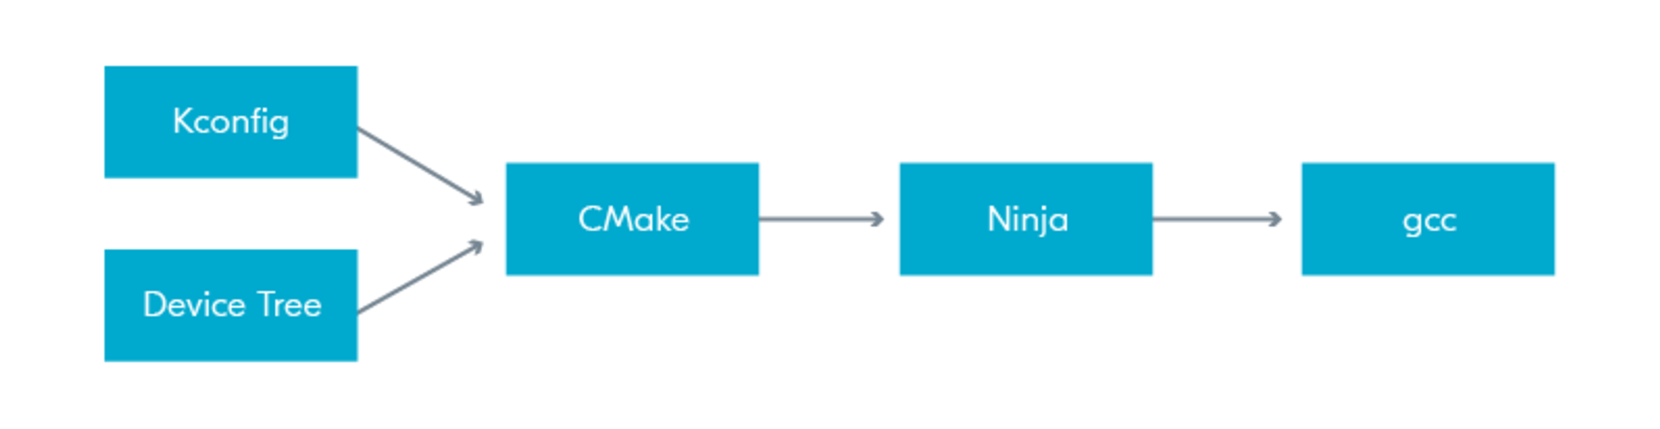
\includegraphics[width=\SchematicWidth]{images/Zephyr/ZephyrBuild.eps}
    \caption{Thread management on the Zephyr RTOS}
\end{figure}
\FloatBarrier

In this image, KConfig refer to the software configuration files, that include 
drivers selections and so. This file is linked to the devicetree, because to 
exploit a peripheral, we need to enable it in hardware, but we also need the associated
drivers with it.

To give an example, this kind of files look like : 
\inputminted[linenos, firstline=32, lastline=70]{kconfig}{data/code/cfg/prj.conf}

Thats basically a list of variable that we set to enable, or disable a software driver.

\subsection{Tasks management}
Zephyr does the task management in a different way other RTOS would. It is not bound to 
the fixed interval timer that would trigger a scheduling every period. This RTOS use the
task as self-scheduling.

\begin{figure}[!hbt]
    \centering
    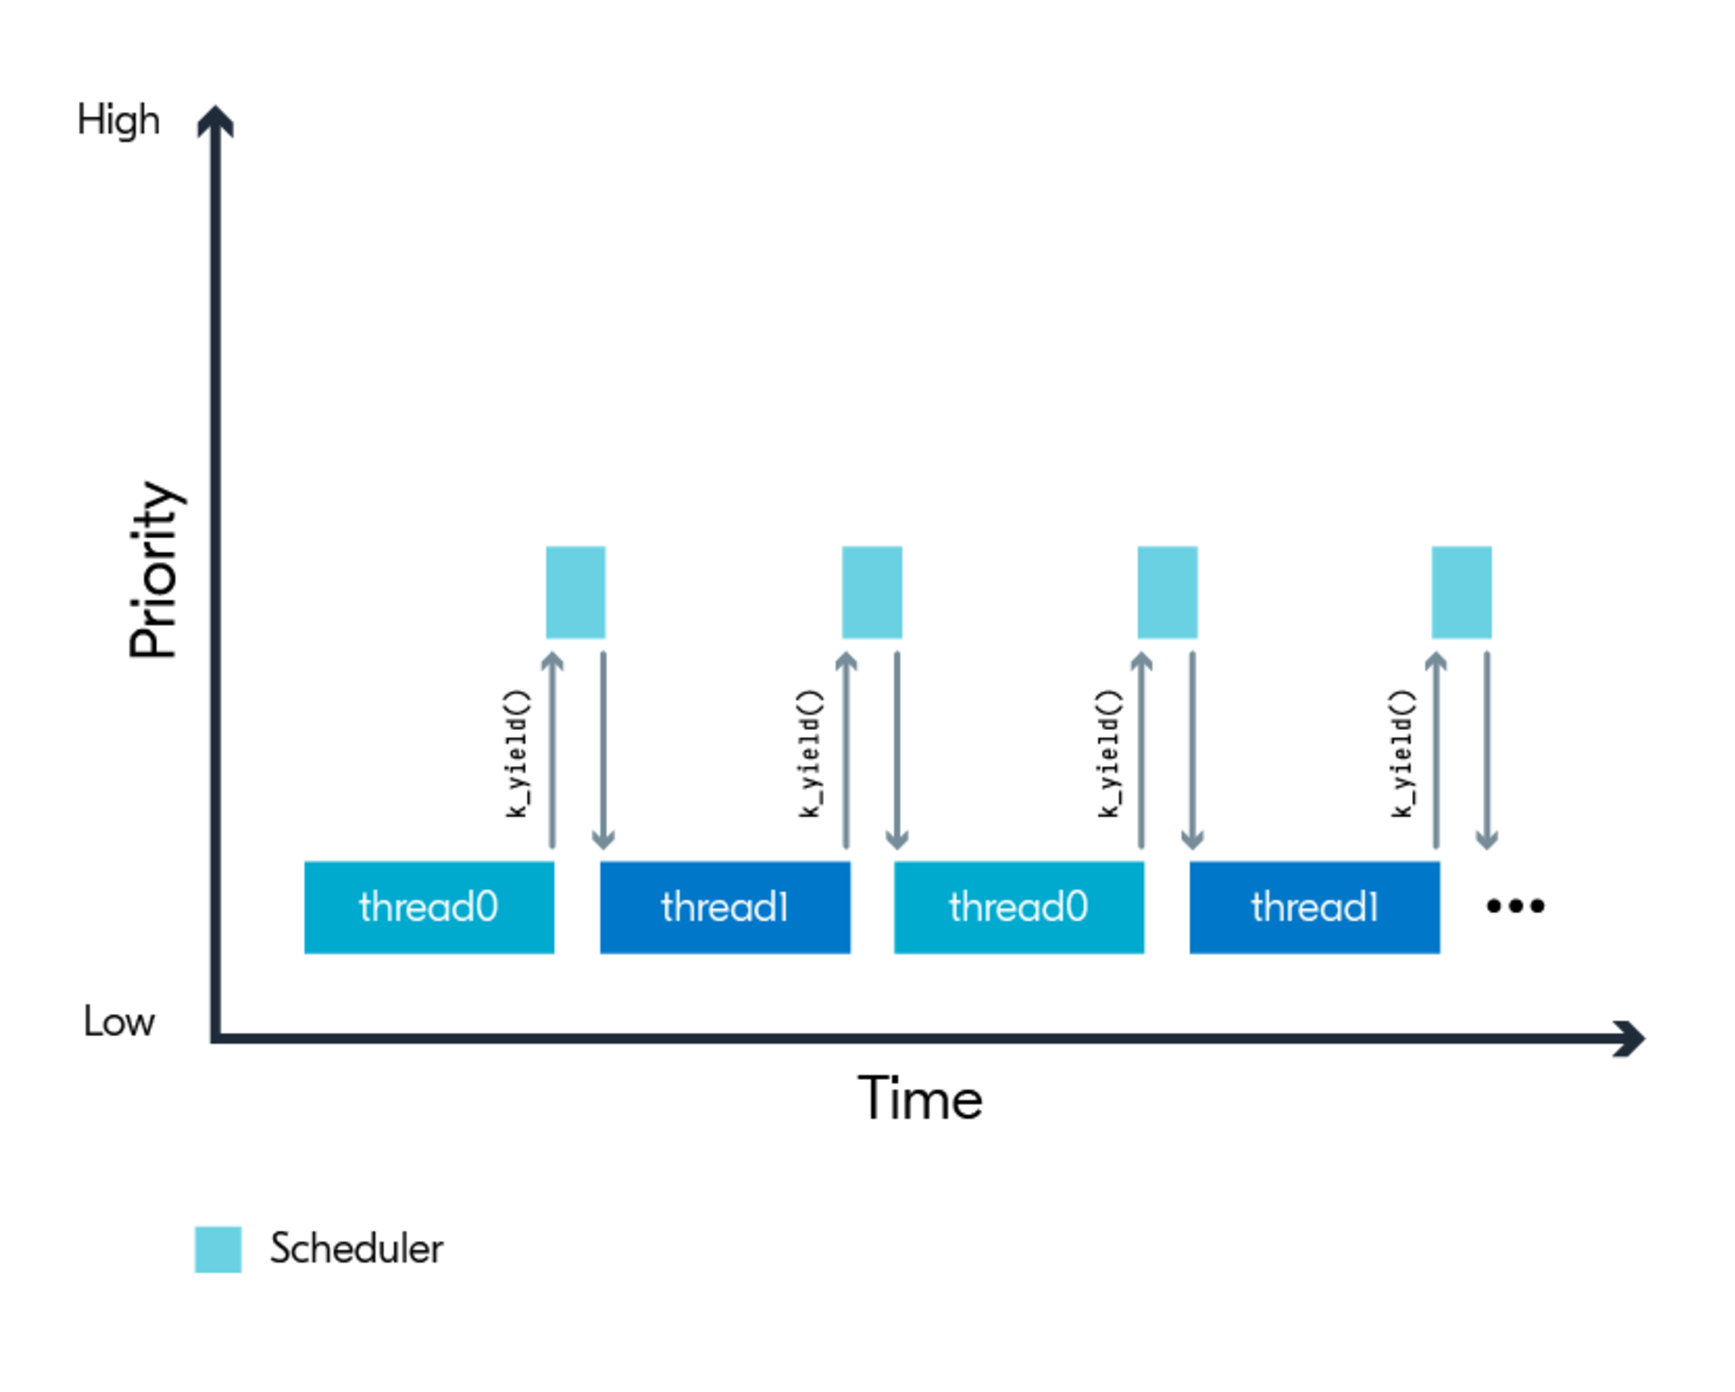
\includegraphics[width=\SchematicWidth]{images/Zephyr/ThreadMGNT.eps}
    \caption{Build chain for Zephyr RTOS}
\end{figure}
\FloatBarrier

As we may see on this image, that came from the Nordic training center \cite{NordicFundamentals} 
and \cite{NordicAdvanced} courses, the scheduler is called once a task enter a delay state, or 
yield itself.

On another hand, the RTOS include a safety timer, set to ten milliseconds that will force the
scheduler to be called. This ensure, even if a task enter an infinite loop, or crash, that
the others tasks wont crash.

\subsection{Final words}
To conclude on this RTOS part, we've seen the most basic concepts, but that's enough to
understand how our project is build, and how code interract with other code.

To sum up, Zephyr is an RTOS, used to manage a lot of different things on the project, 
from the most basic configuration of the hardware to the tasks management during the 
execution.


% Drivers
\section{Drivers}
Next in the hierarchy, we found the drivers. This codes are used to prevent from the
user to perform low-level IO, which are error prones.

\paragraph{}
All of them are written by the manufacturer or the chip, in our case, Nordic
Semiconductors.
Theses contain mostly definitions about structures passed to the driver to 
configure an element, of function that we may call.

\subsection{Calling the driver}
Theses drivers can be called by two distinct ways : 
\begin{itemize}
    \item From bare-metal code
    \item From Zephyr RTOS drivers, who redirect calls to the bare-metal code
\end{itemize}

The second method is the safest, in the manner that the RTOS handle the request for us, 
but, to ensure compatibility with a lot of chips, it can't provide exact same options as
the bare metal driver.

That's why we used both, mostly the Zephyr one were we could.

\subsection{Driver usage}
\subsubsection{Bare metal}
To give an example of the driver beeing used, there is the initialization code the ADC module 

\inputminted[linenos, firstline=103, lastline=112]{cpp}{data/code/C/saadc.cpp}

This code is responsible for the configuration of some advanced behaviors of the ADC peripheral,
such as setting it's resolution, callback function and so.
Calls are here quite long, because of the different structs that need to be configured, defined,
and applied for each aspect.

\subsubsection{Zephyr}

On the other hand, here the example for the Zephyr driver being called.
This is much simpler, because we're here calling the Zephyr Driver that handle a lot of the work 
for us, based on the devicetree !

\inputminted[linenos, firstline=100, lastline=102]{cpp}{data/code/C/servo.cpp}

We just need to care about the pulse length we want to set. All the other parameters were defined
when the kernel was booting.







\input{chapters/prog/HAL/device-drivers.tex}

% Gloval architecute
\input{chapters/prog/architecture/architecture.tex}
